\documentclass[]{article}
\usepackage{lmodern}
\usepackage{amssymb,amsmath}
\usepackage{ifxetex,ifluatex}
\usepackage{fixltx2e} % provides \textsubscript
\ifnum 0\ifxetex 1\fi\ifluatex 1\fi=0 % if pdftex
  \usepackage[T1]{fontenc}
  \usepackage[utf8]{inputenc}
\else % if luatex or xelatex
  \ifxetex
    \usepackage{mathspec}
  \else
    \usepackage{fontspec}
  \fi
  \defaultfontfeatures{Ligatures=TeX,Scale=MatchLowercase}
\fi
% use upquote if available, for straight quotes in verbatim environments
\IfFileExists{upquote.sty}{\usepackage{upquote}}{}
% use microtype if available
\IfFileExists{microtype.sty}{%
\usepackage[]{microtype}
\UseMicrotypeSet[protrusion]{basicmath} % disable protrusion for tt fonts
}{}
\PassOptionsToPackage{hyphens}{url} % url is loaded by hyperref
\usepackage[unicode=true]{hyperref}
\hypersetup{
            pdftitle={Gerber and Green Experiment},
            pdfborder={0 0 0},
            breaklinks=true}
\urlstyle{same}  % don't use monospace font for urls
\usepackage{longtable,booktabs}
% Fix footnotes in tables (requires footnote package)
\IfFileExists{footnote.sty}{\usepackage{footnote}\makesavenoteenv{long table}}{}
\usepackage{graphicx,grffile}
\makeatletter
\def\maxwidth{\ifdim\Gin@nat@width>\linewidth\linewidth\else\Gin@nat@width\fi}
\def\maxheight{\ifdim\Gin@nat@height>\textheight\textheight\else\Gin@nat@height\fi}
\makeatother
% Scale images if necessary, so that they will not overflow the page
% margins by default, and it is still possible to overwrite the defaults
% using explicit options in \includegraphics[width, height, ...]{}
\setkeys{Gin}{width=\maxwidth,height=\maxheight,keepaspectratio}
\IfFileExists{parskip.sty}{%
\usepackage{parskip}
}{% else
\setlength{\parindent}{0pt}
\setlength{\parskip}{6pt plus 2pt minus 1pt}
}
\setlength{\emergencystretch}{3em}  % prevent overfull lines
\providecommand{\tightlist}{%
  \setlength{\itemsep}{0pt}\setlength{\parskip}{0pt}}
\setcounter{secnumdepth}{5}
% Redefines (sub)paragraphs to behave more like sections
\ifx\paragraph\undefined\else
\let\oldparagraph\paragraph
\renewcommand{\paragraph}[1]{\oldparagraph{#1}\mbox{}}
\fi
\ifx\subparagraph\undefined\else
\let\oldsubparagraph\subparagraph
\renewcommand{\subparagraph}[1]{\oldsubparagraph{#1}\mbox{}}
\fi

% set default figure placement to htbp
\makeatletter
\def\fps@figure{htbp}
\makeatother


\title{Gerber and Green Experiment}
\date{}

\begin{document}
\maketitle

\section{Gerber and Green (2003)}\label{gerber-and-green-2003}

In this appendix, I first describe the experimental data from the paper.
The original sample size for the experiment consists of 18933
individuals from 6 different cities in the United States.

\subsection{Data preparation}\label{data-preparation}

\subsubsection{Variables}\label{variables}

The dependent variable \texttt{voted00} tells us whether the person
voted in the 6 November election in 2001. The treatment indicator
\texttt{treatmen} tells us whether the individual was encouraged to be
visited by the canvassers. Additionally, the experiment records six
background variables about every individual; race, sex, age, party
affiliation, turnout in the 2000 election and turnout in the 1999
election.

In our prediction problem using the experimental data, we do not use the
1999 election variable. According to our knowledge, no elections ocurred
in all of the concerned cities in 1999.

\subsubsection{Missing data}\label{missing-data}

There is missing data in the experimental data. In R, the missing data
was first recoded to the R's standard NA format and the patterns are
visualised in the Figure ().

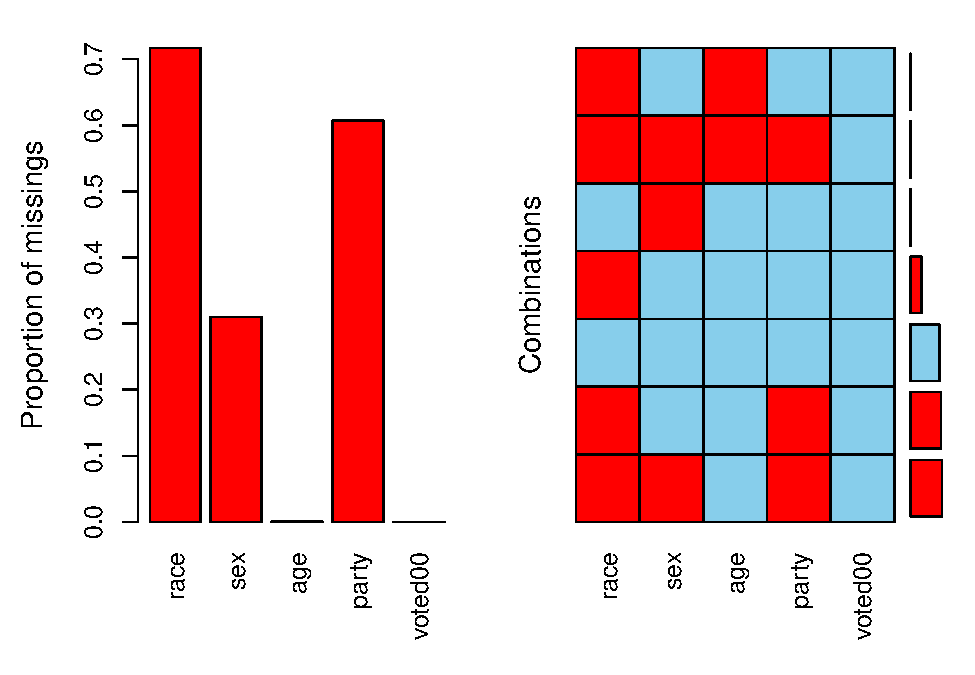
\includegraphics{GerberGreen_Appendix_files/figure-latex/Aggregate plot for missingness-1.pdf}

Rather than looking at aggregate patterns of missingness, what is more
of an interest for our specific case are the patterns of missing values
in each of the locations. We proceed with complete case analysis for
cases where the missingness is \textasciitilde{}1\% on a covariate for a
given location. The table below shows the proportion of missing values
for a given covariate for every location.

\begin{longtable}[]{@{}lrrrrr@{}}
\toprule
& race & sex & age & party & voted00\tabularnewline
\midrule
\endhead
Raleigh & 0 & 0.30 & 0.00 & 0 & 0\tabularnewline
Bridgeport & 100 & 0.00 & 0.11 & 0 & 0\tabularnewline
Detroit & 100 & 1.11 & 0.00 & 100 & 0\tabularnewline
Minneapolis & 100 & 100.00 & 0.00 & 100 & 0\tabularnewline
St Paul & 100 & 100.00 & 0.32 & 100 & 0\tabularnewline
\bottomrule
\end{longtable}

In the complete case analysis we dicarded 78 rows from the dataset.

\subsubsection{Other data
transformations}\label{other-data-transformations}

As the next step in the data transformation process, we delete one
invalid data observation with the value of 2001 for age.

Additionally, we reclassify subjects who answered with Unknown to their
sex to `NA' and excluded. This simplifies the matching procedure since
with only two sexes, the variable can be operationalised as a dummy
variable.

\subsection{Data exploration}\label{data-exploration}

\subsubsection{The varying individual characteristics between
locations}\label{the-varying-individual-characteristics-between-locations}

This

\paragraph{Age and Voting in the 2000
election}\label{age-and-voting-in-the-2000-election}

\begin{longtable}[]{@{}lrrrrr@{}}
\toprule
& Raleigh & Bridgeport & Detroit & Minneapolis & St Paul\tabularnewline
\midrule
\endhead
age & 45.61 & 44.78 & 49.35 & 39.66 & 41.72\tabularnewline
voted00 & 0.72 & 0.44 & 0.61 & 0.54 & 0.82\tabularnewline
\bottomrule
\end{longtable}

\paragraph{Sex}\label{sex}

\begin{longtable}[]{@{}lrrr@{}}
\toprule
& F & M & U\tabularnewline
\midrule
\endhead
Raleigh & 0.51 & 0.49 & NA\tabularnewline
Bridgeport & 0.61 & 0.38 & 0.01\tabularnewline
Detroit & 0.61 & 0.39 & NA\tabularnewline
\bottomrule
\end{longtable}

\paragraph{Party affiliation}\label{party-affiliation}

\begin{longtable}[]{@{}lrrr@{}}
\toprule
& D & I & R\tabularnewline
\midrule
\endhead
Raleigh & 0.48 & 0.20 & 0.31\tabularnewline
Bridgeport & 0.54 & 0.38 & 0.08\tabularnewline
\bottomrule
\end{longtable}

\subsection{Further causalMatch
specifications}\label{further-causalmatch-specifications}

In the operationalisation of causalMatch to the experimental data in the
dissertation we have rescaled the age variable to be in the range 0 to
1. Here, I provide two other additional options of working with the
variable. First, I scale the age variable by dividing it by its
root-mean-square defined as \(\sqrt{\frac{1}{n}\sum_{t=1}^{n}age_t^2}\).
The results can be seen in the table below.

\begin{longtable}[]{@{}lrrrrr@{}}
\toprule
& \(\tau_{ITT}^{PRED}\) & \(\hat{\tau_{ITT}}\) & SE &
\(\tau_{ITT}^{NAIVE}\) & NPE\tabularnewline
\midrule
\endhead
Bridgeport & 2.29 & 3.84 & 2.42 & 2.01 & 3.37\tabularnewline
Raleigh & 2.76 & -0.90 & 13.38 & 3.19 & 16.77\tabularnewline
Detroit & 1.56 & 2.47 & 0.83 & 2.35 & 0.02\tabularnewline
Minneapolis & 3.46 & 1.99 & 2.18 & 2.47 & 0.23\tabularnewline
St Paul & 3.65 & 4.47 & 0.67 & 1.85 & 6.87\tabularnewline
\bottomrule
\end{longtable}

Finally, the table below presents the unscaled results. In this case, no
transformation was applied to the age variable.

\begin{longtable}[]{@{}lrrrrr@{}}
\toprule
& \(\tau_{ITT}^{PRED}\) & \(\hat{\tau_{ITT}}\) & SE &
\(\tau_{ITT}^{NAIVE}\) & NPE\tabularnewline
\midrule
\endhead
Bridgeport & 2.97 & 3.84 & 0.77 & 2.01 & 3.37\tabularnewline
Raleigh & 2.91 & -0.90 & 14.57 & 3.19 & 16.77\tabularnewline
Detroit & 1.68 & 2.47 & 0.63 & 2.35 & 0.02\tabularnewline
Minneapolis & 3.45 & 1.99 & 2.14 & 2.47 & 0.23\tabularnewline
St Paul & 3.63 & 4.47 & 0.70 & 1.85 & 6.87\tabularnewline
\bottomrule
\end{longtable}

Compared to the table presented in the main body of the dissertation
(see Table ), the different specification of scaling does not alter our
conclusion that we can predict the ITT more accurately than using the
naive method in four out of six cases.

\end{document}
